Dans un repère orthogonal, donnons nous l'hyperbole $\setgeo{H} : y = \frac{1}{x}$ . Plaçons-y les points $A$ , $B$ et $P$ d'abscisses respectives $a$ , $b$ et  $p = ab$ .
Observez
\footnote{
	Pour conjecturer plus facilement quelque chose, utilisez le fichier GeoGebra \texttt{base-tool.ggb} manipulable dynamiquement qui est disponible sur le lieu de téléchargement de ce document.
}
les trois cas ci-dessous et essayez de conjecturer quelque chose \emph{(la réponse est donnée dans la page suivante)}
\footnote{
	On sait \emph{\og additionner \fg} sur un cercle et sur $\setgeo{P} : y = x^2$ .
	Or $yx$ , $x^2 - y^2$ et $x^2 - y$ sont des formes quadratiques qui ont des propriétés géométriques communes.
	Avec tout ceci en tête, la recherche proposée ici devient très naturelle.
}.


\begin{center}
	\footnotesize
	\itshape

	\fbox{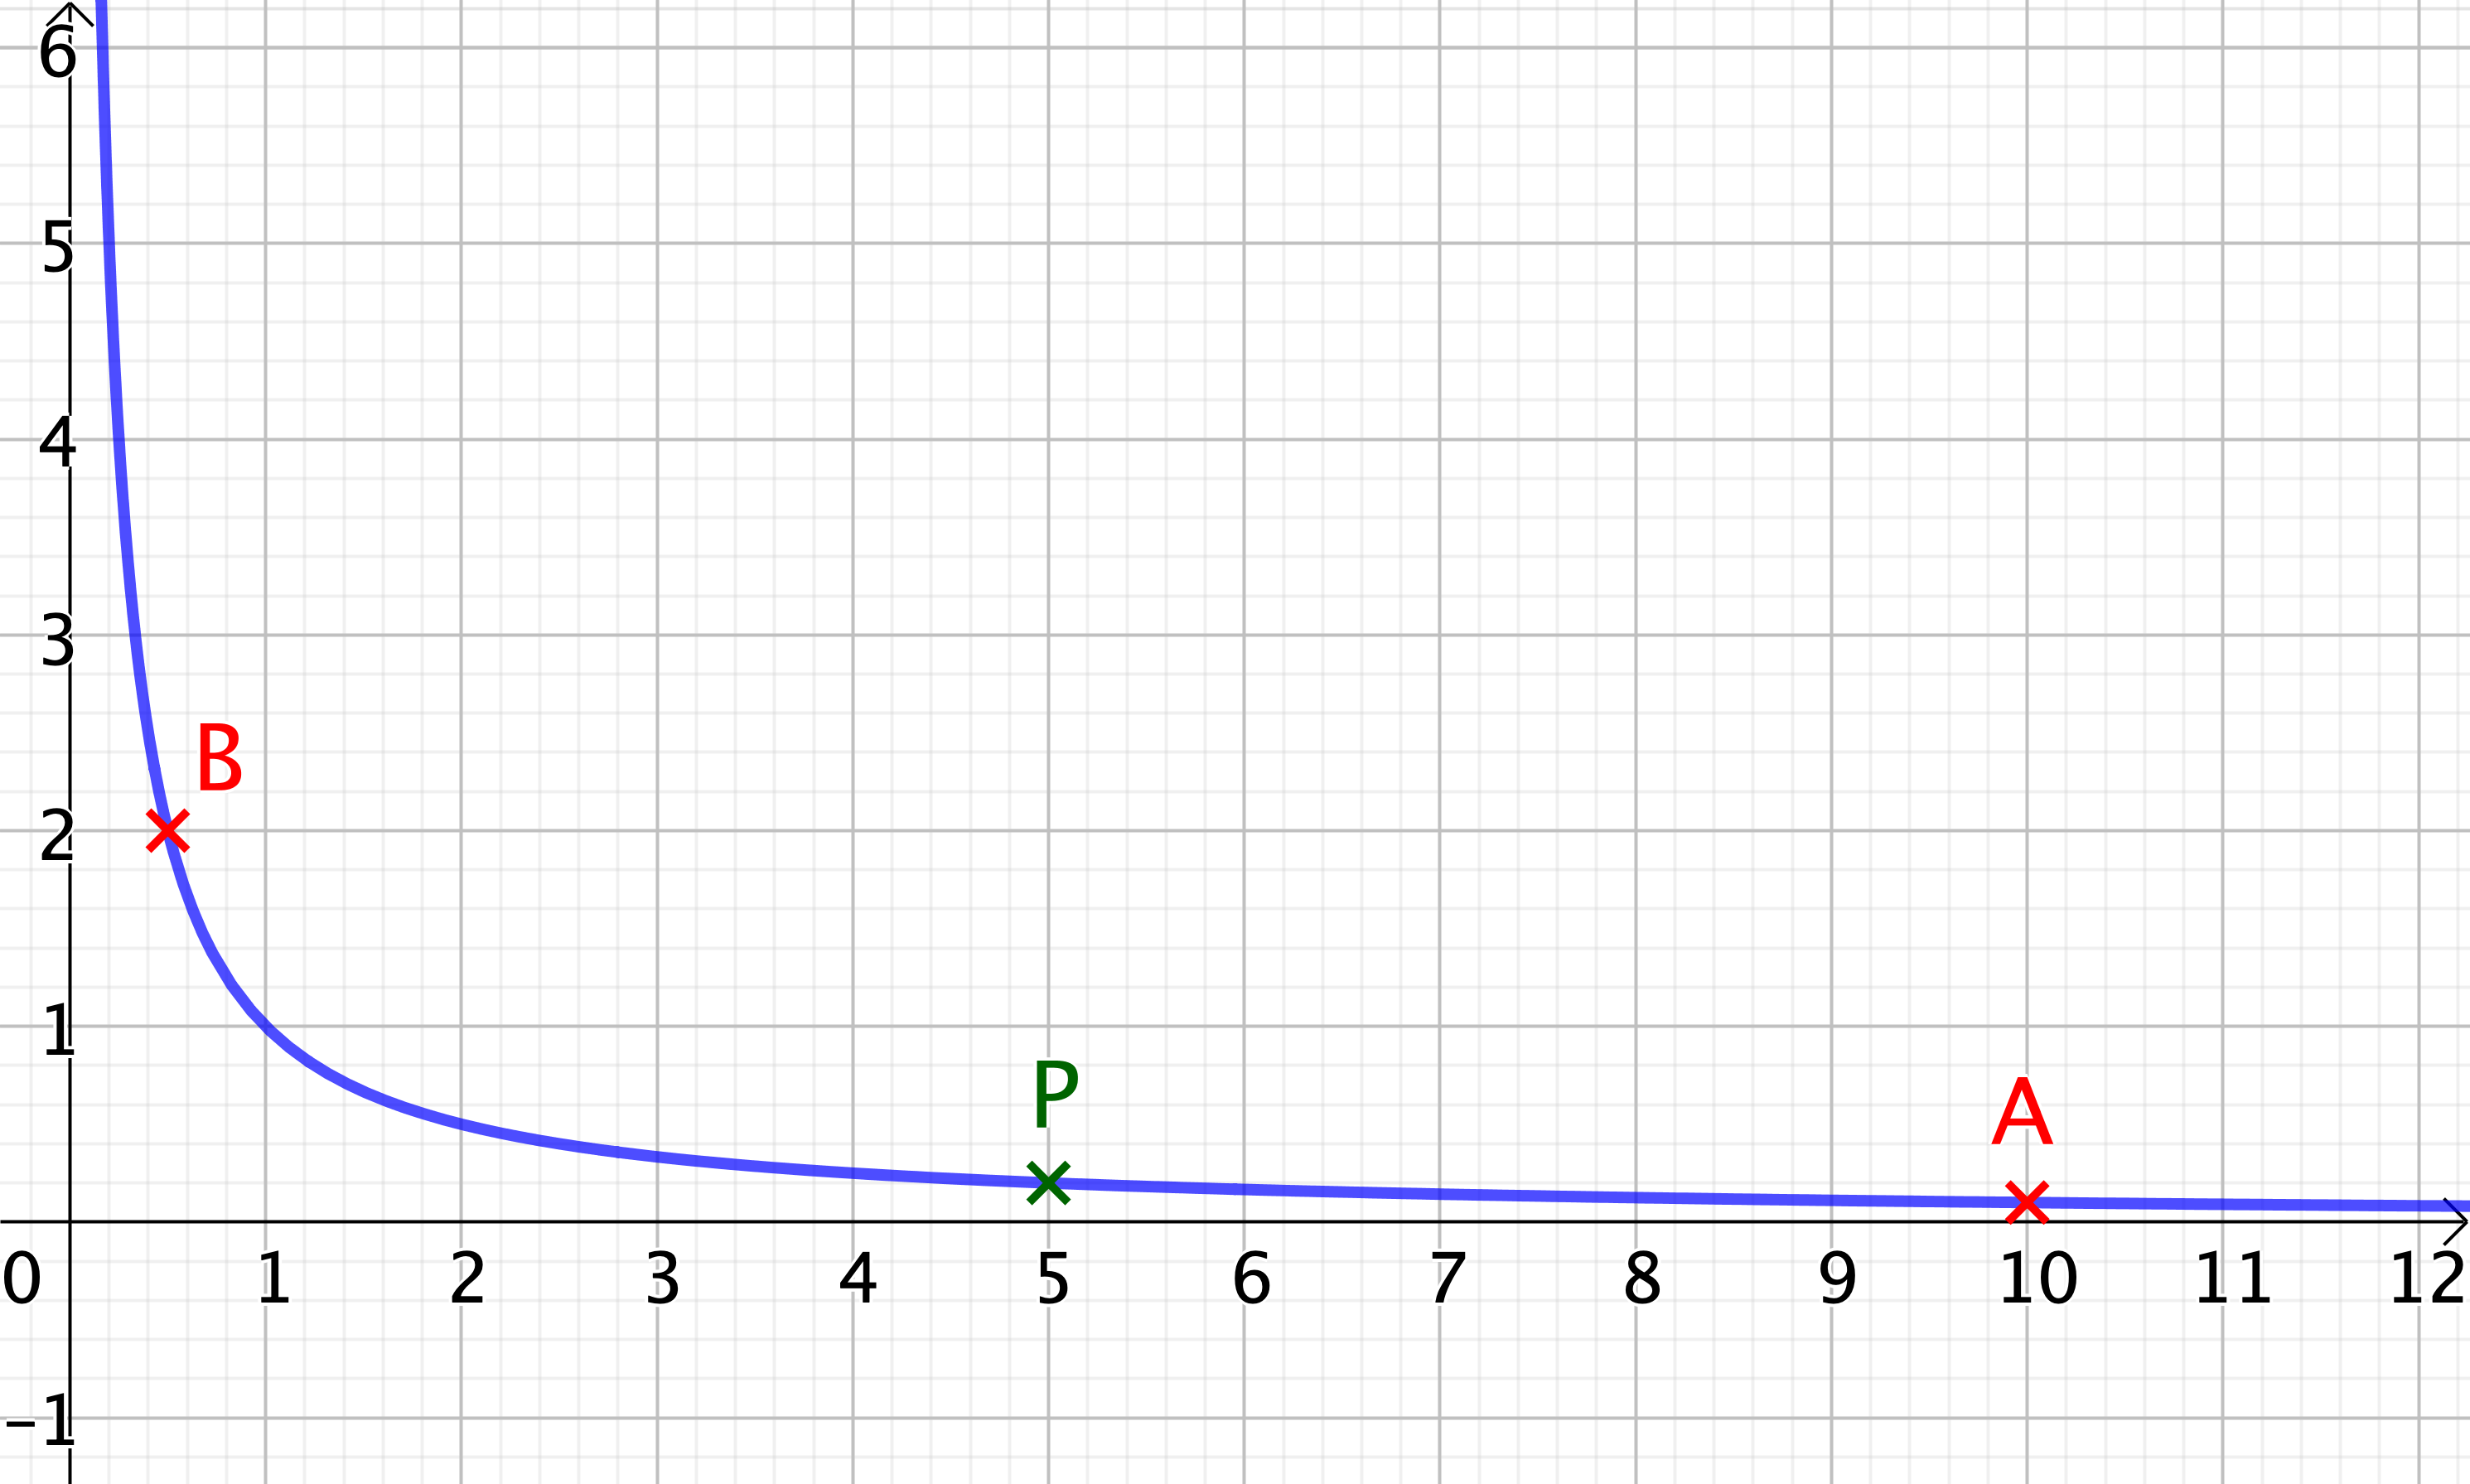
\includegraphics[scale = .75]{product-on-hyperbolas/conjecture/a-and-b-positive.png}}
	
	\smallskip
	Cas où $a > 0$ et $b > 0$

	\medskip
	
	\fbox{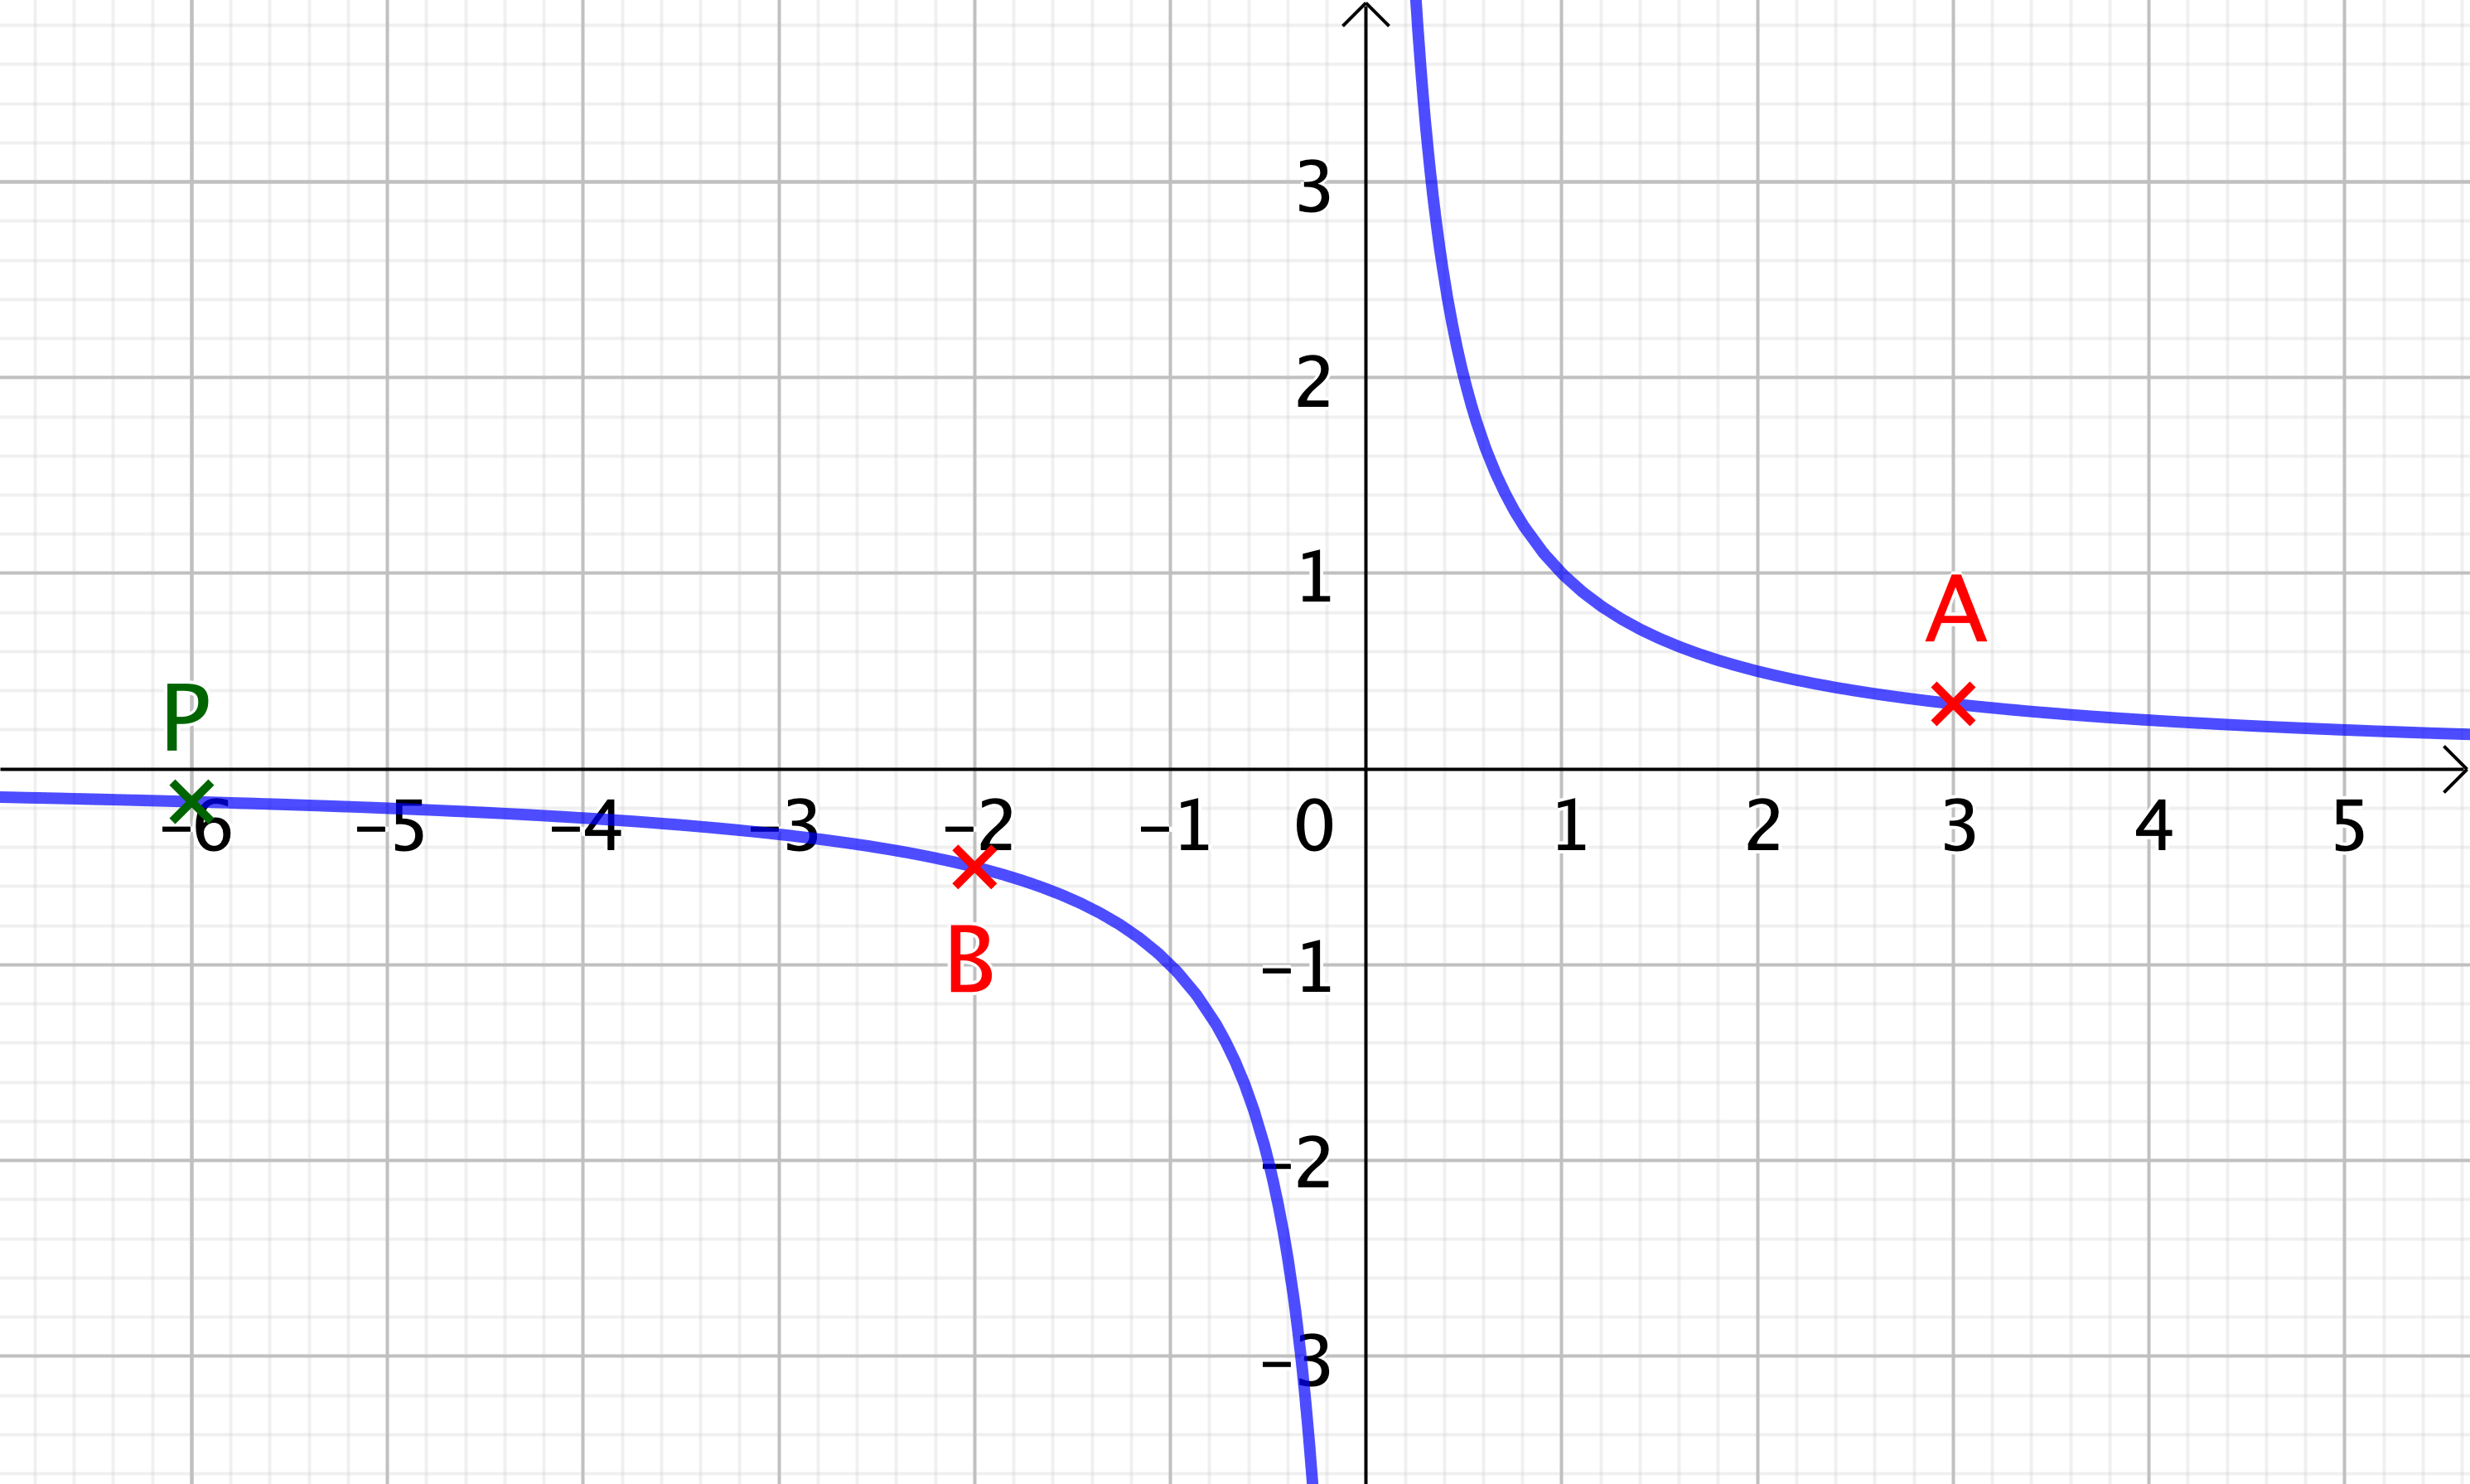
\includegraphics[scale = .75]{product-on-hyperbolas/conjecture/a-and-b-diff-signs.png}}
	
	\smallskip
	Cas où $a < 0$ et $b > 0$

	\medskip

	\fbox{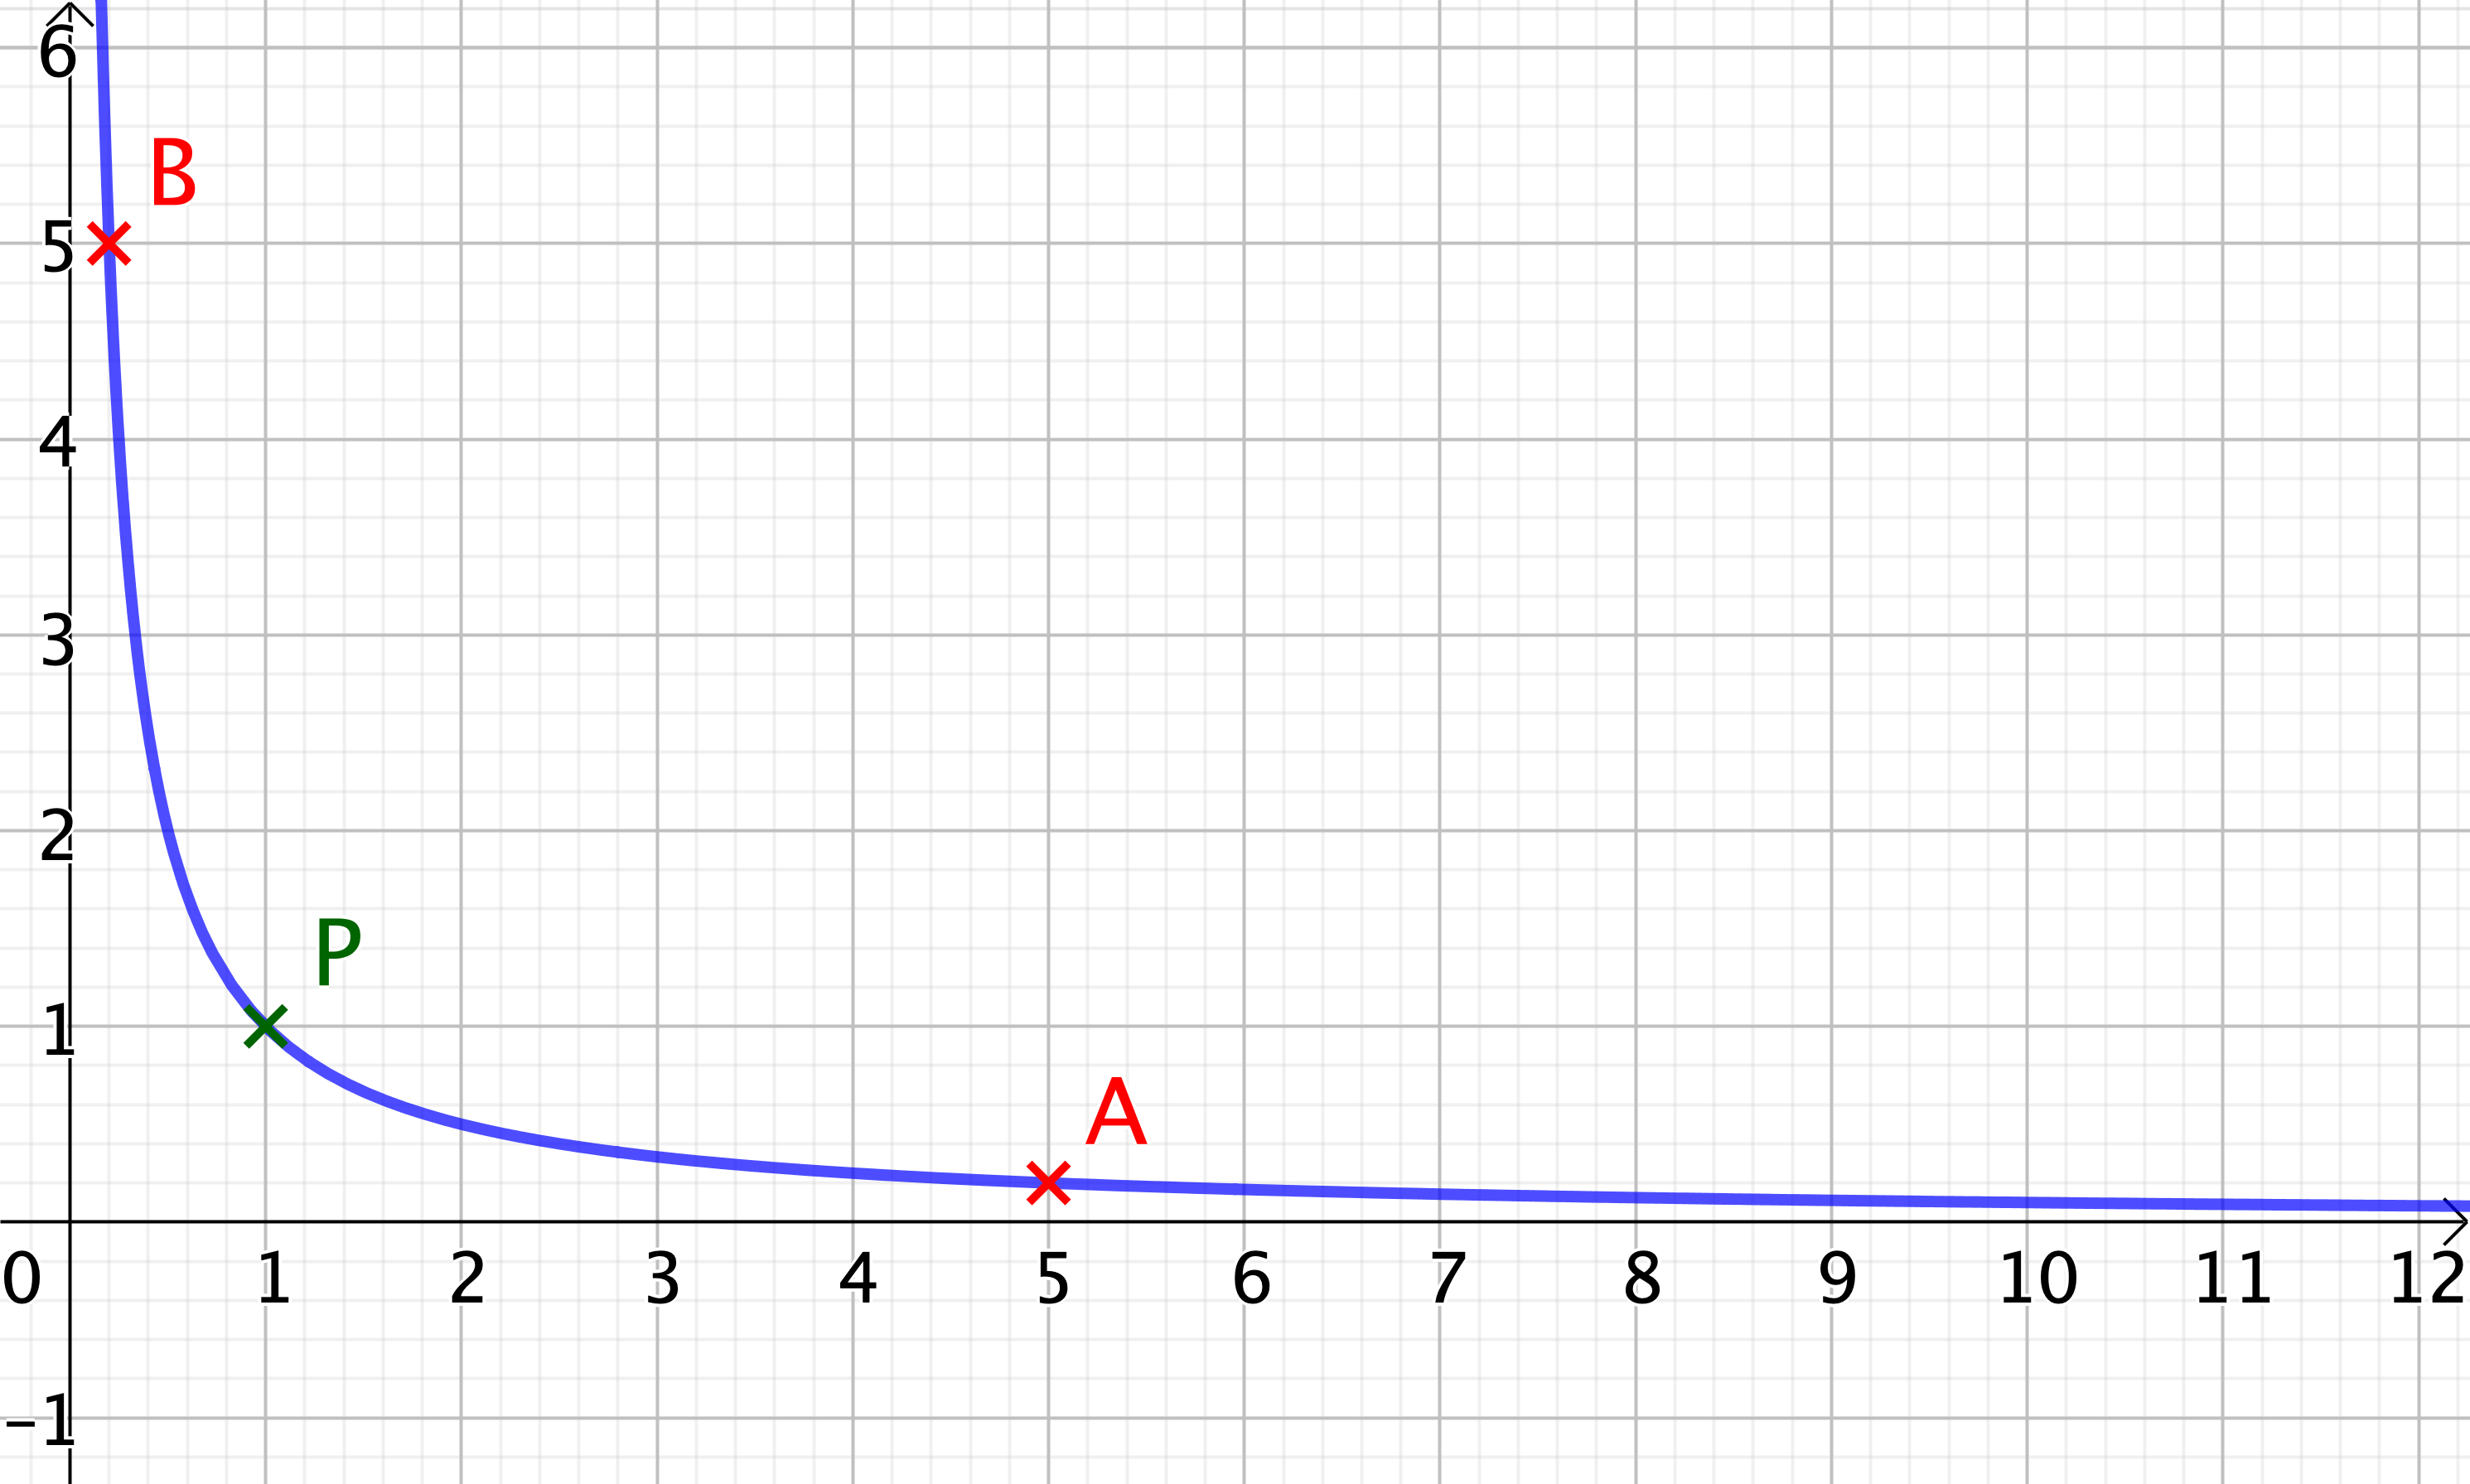
\includegraphics[scale = .75]{product-on-hyperbolas/conjecture/a-and-b-inverse.png}}
	
	\smallskip
	Cas où $a b = 1$
\end{center}


\newpage

Pour mieux voir ce qu'il se passe, ajoutons $E(1 ; 1)$ , ce qui semble naturel car $1$ est son propre inverse, et traçons quelques droites. Voici ce que cela donne.

\begin{center}
	\footnotesize
	\itshape

	\fbox{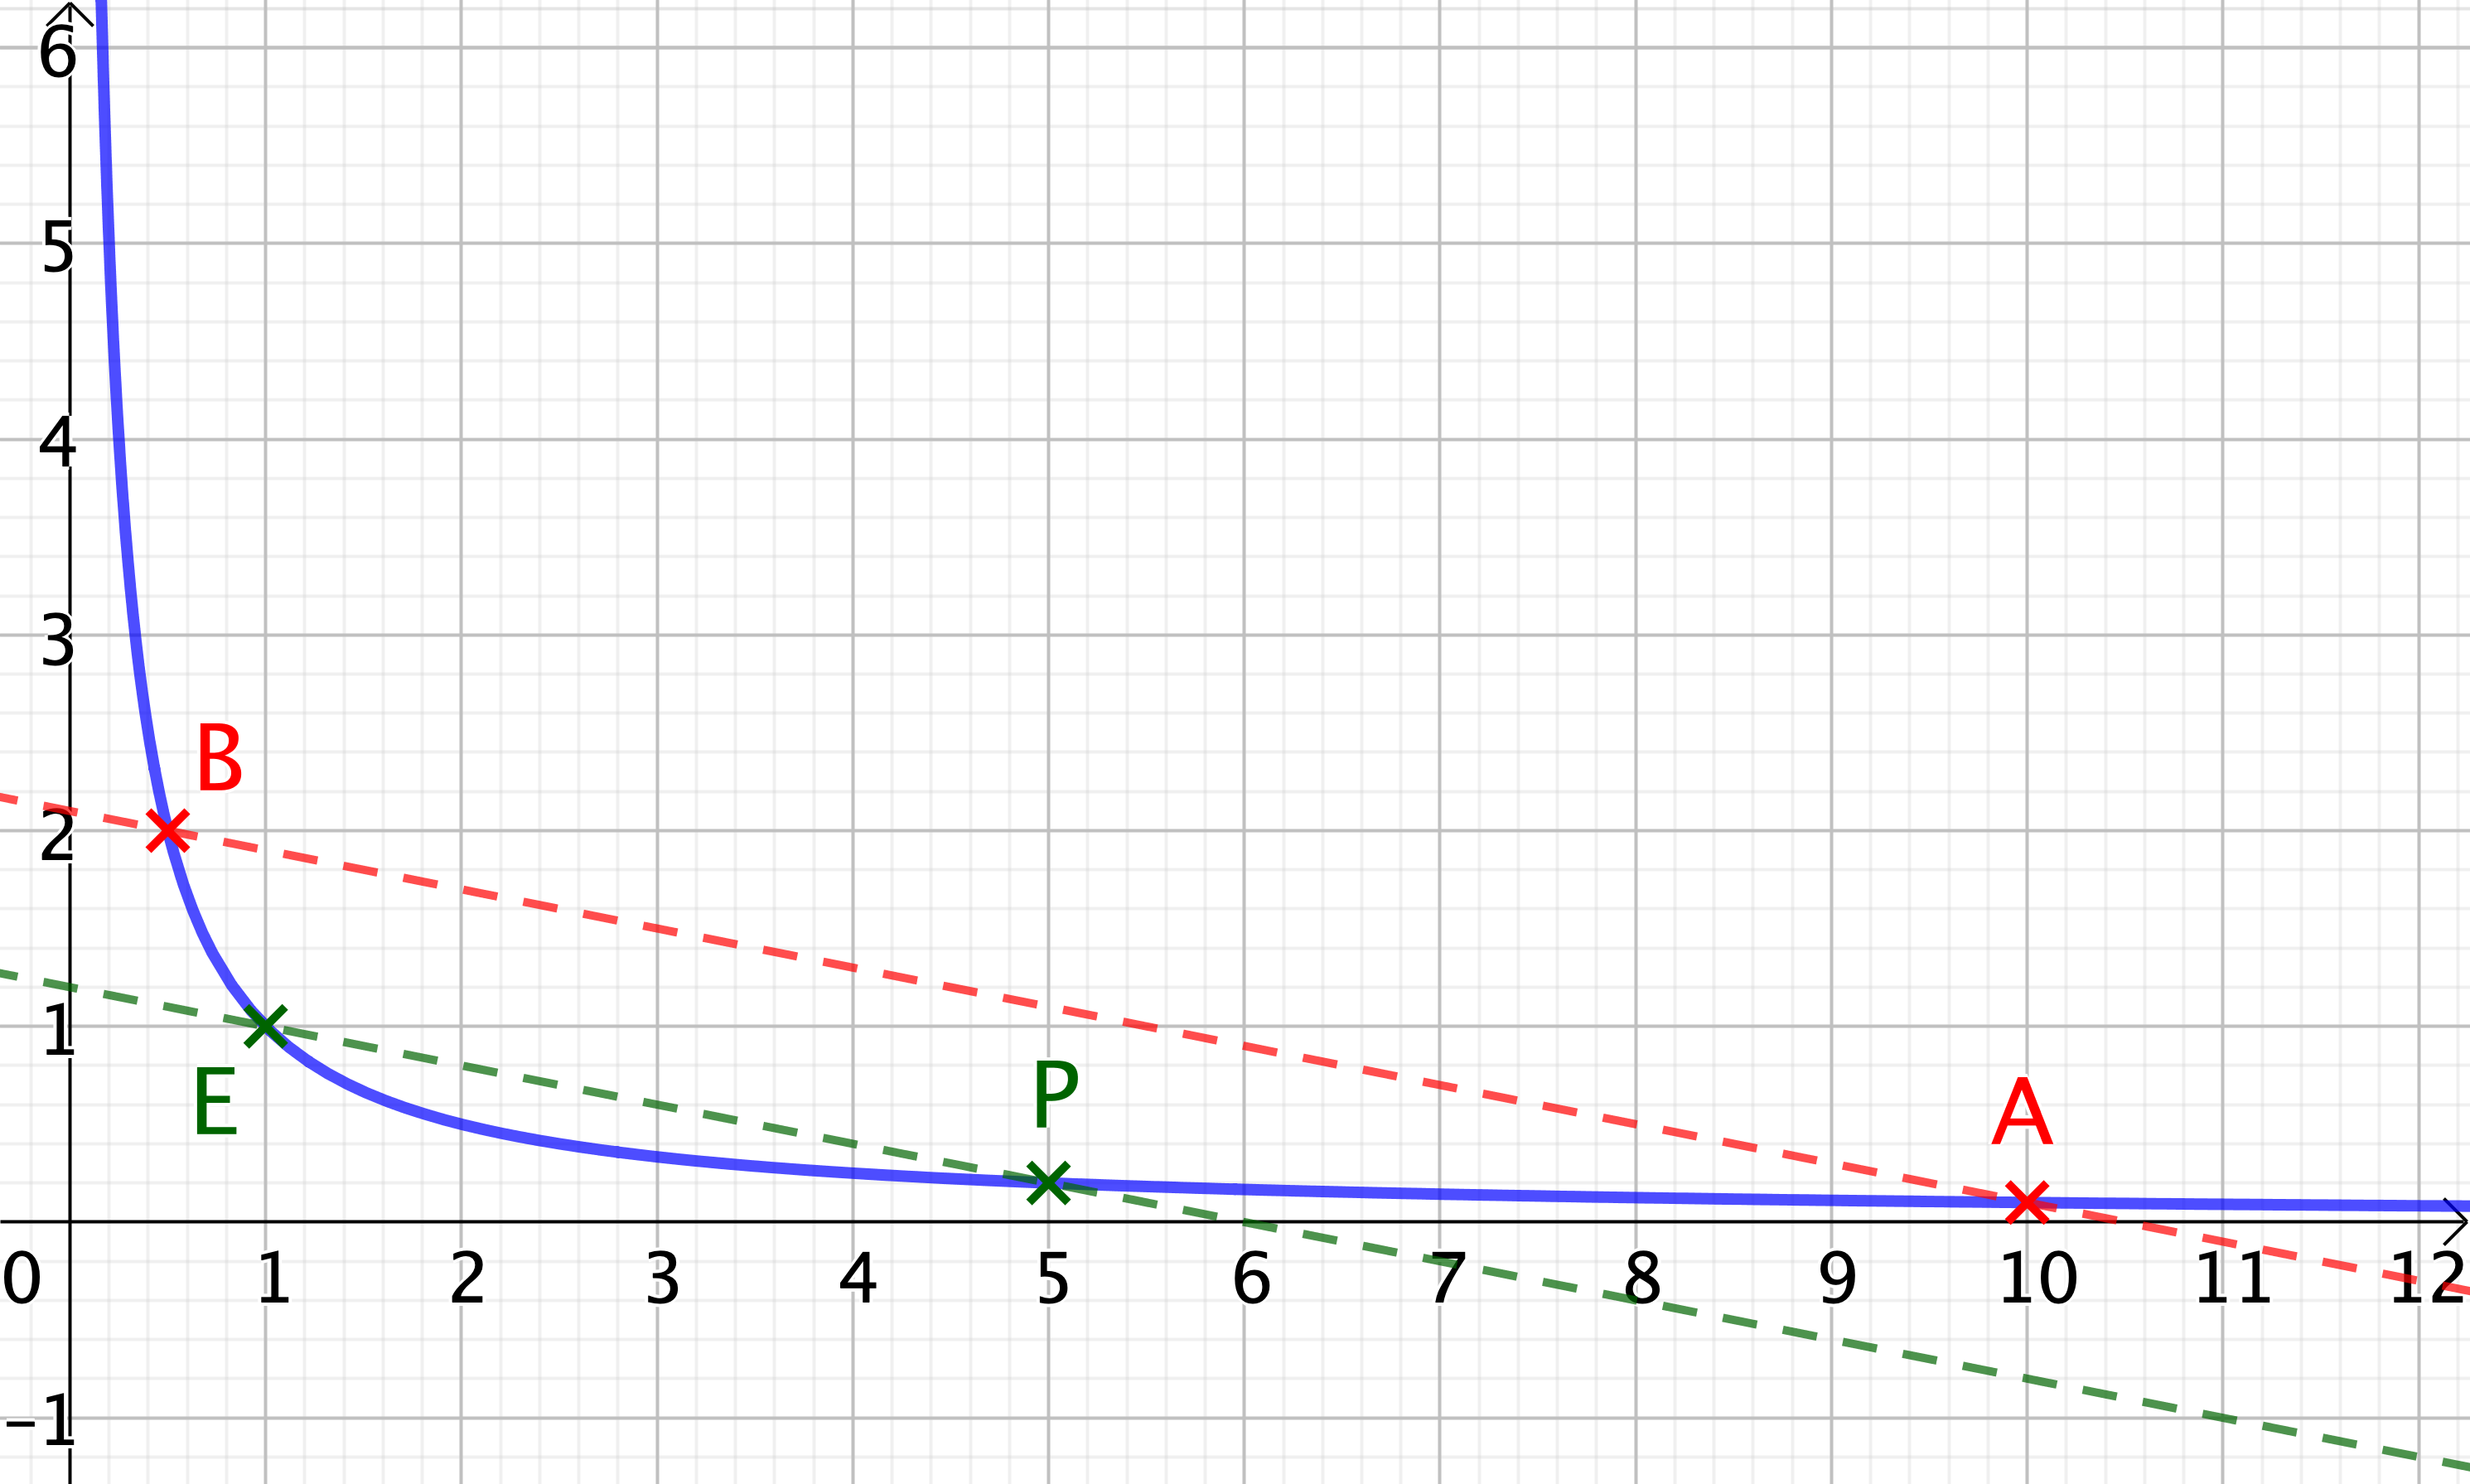
\includegraphics[scale = .75]{product-on-hyperbolas/conjecture/a-and-b-positive-with-lines.png}}
	
	\smallskip
	Cas où $a > 0$ et $b > 0$

	\medskip

	\fbox{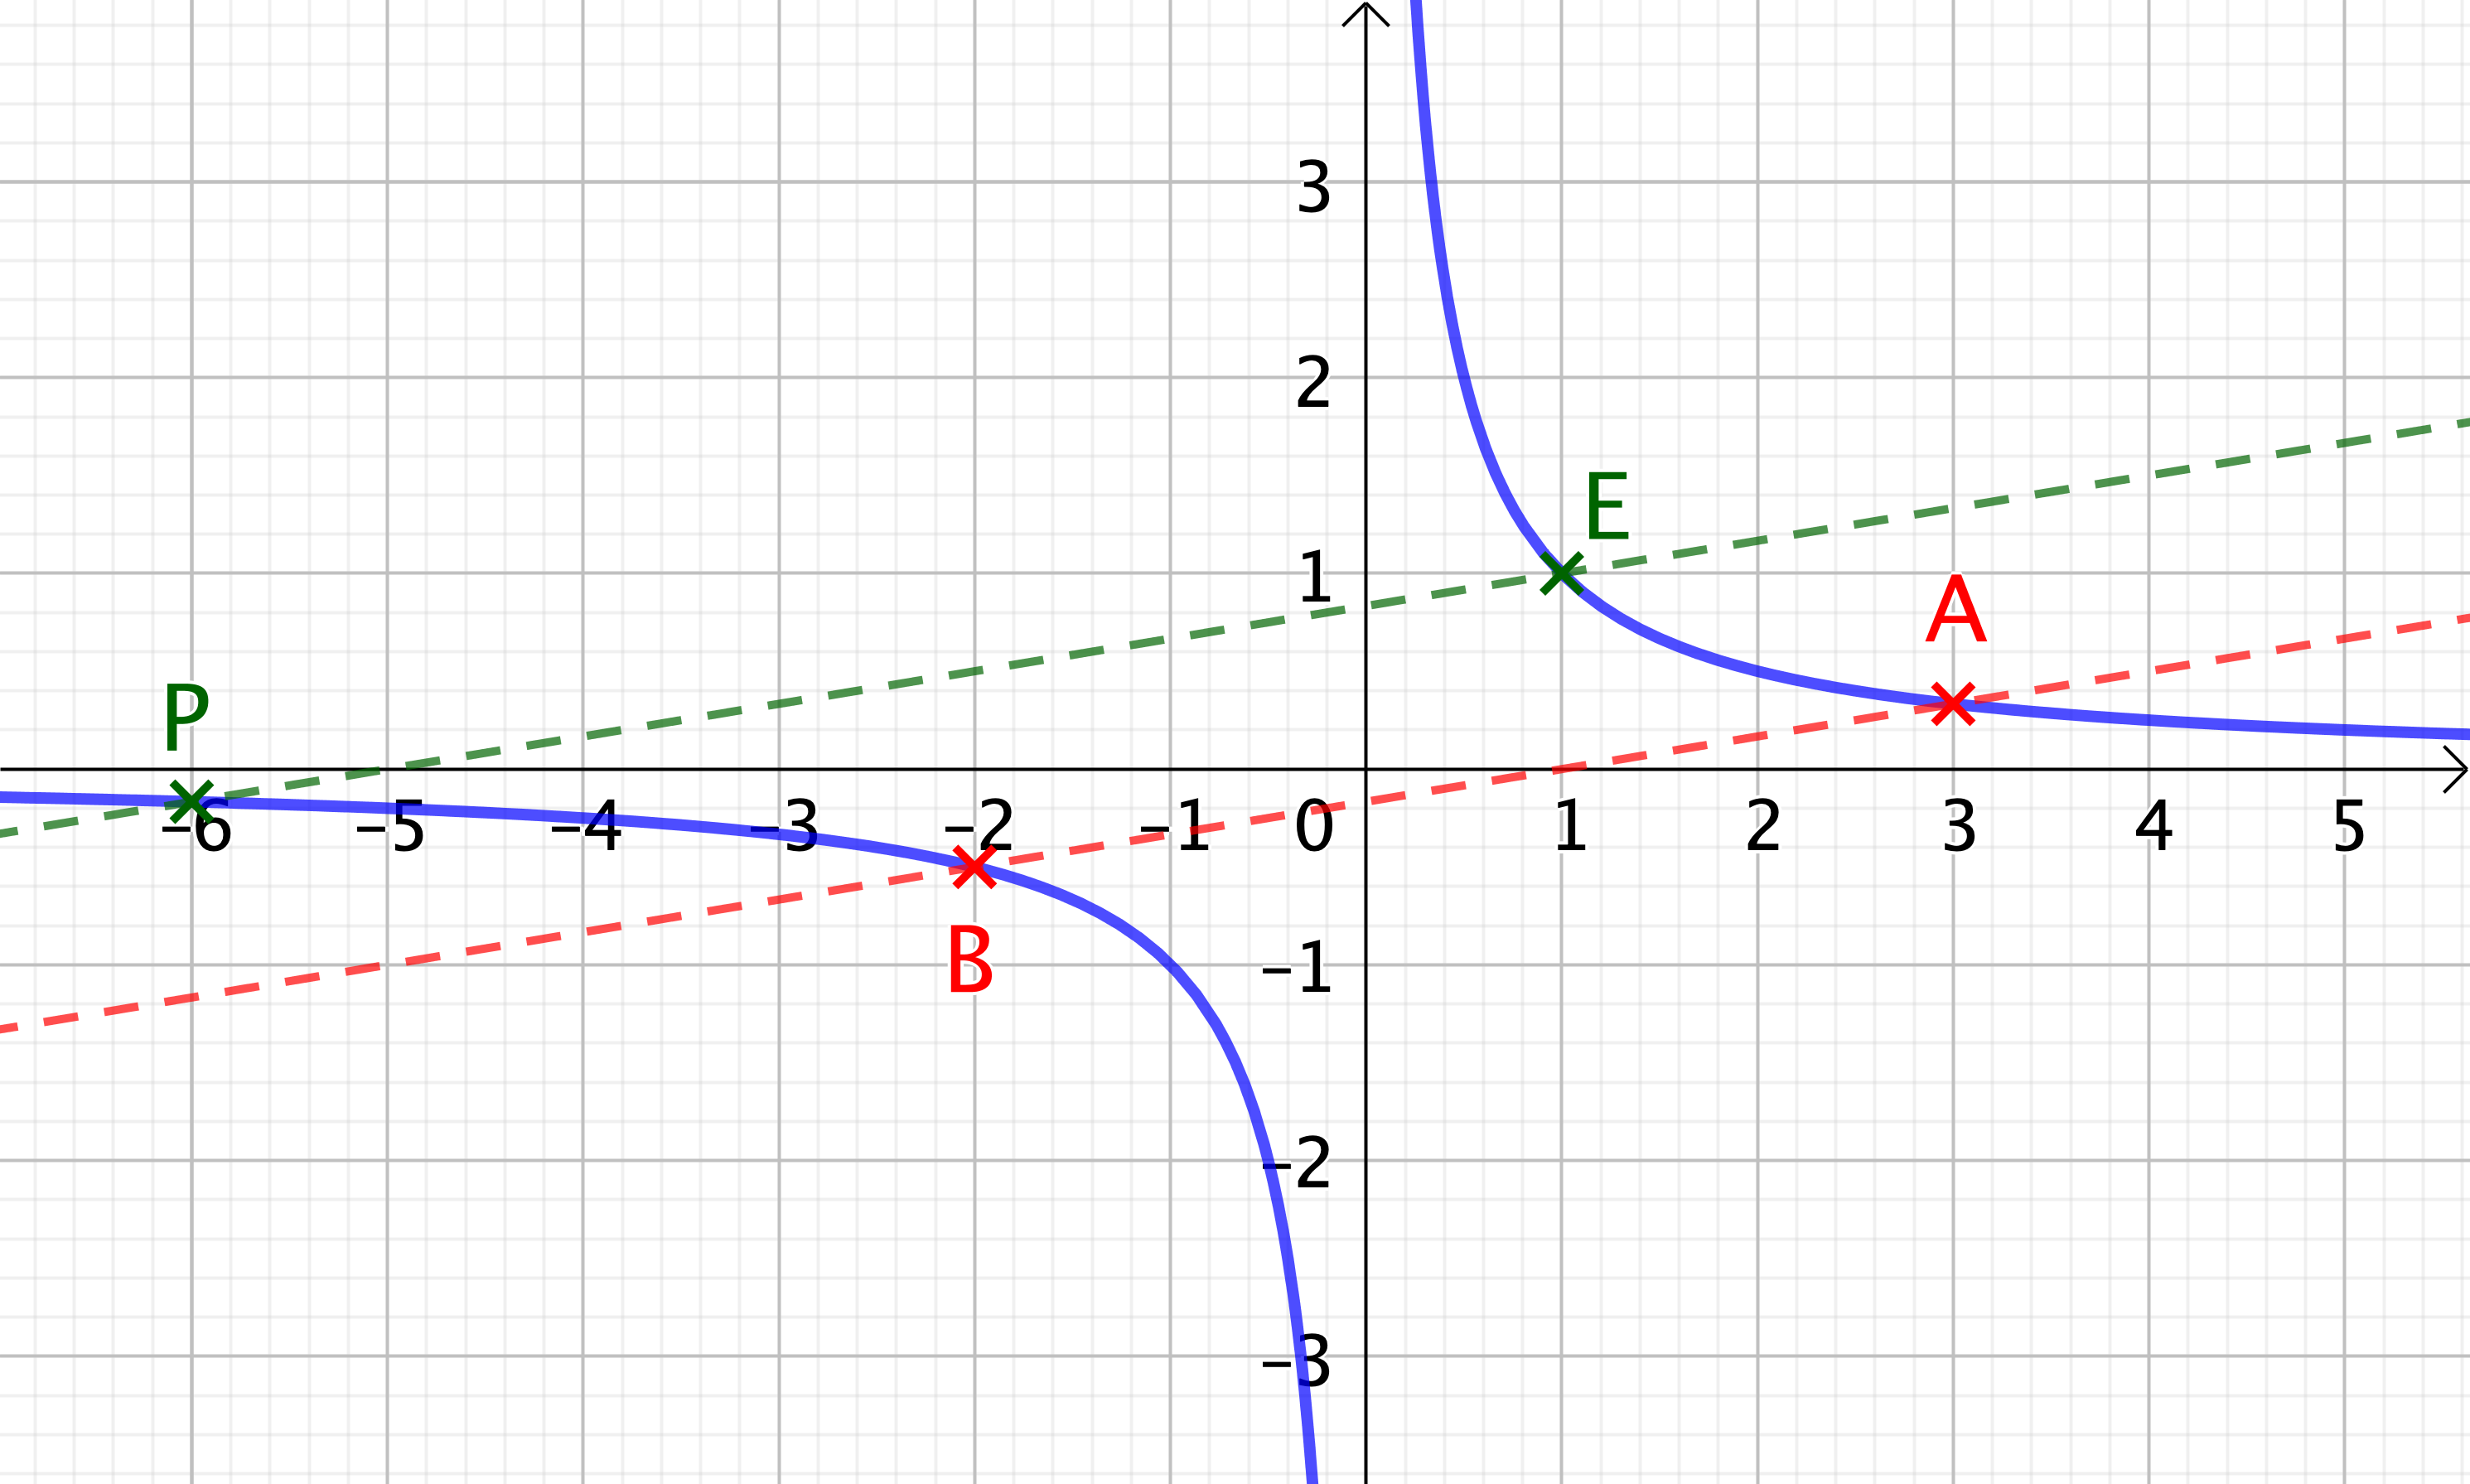
\includegraphics[scale = .75]{product-on-hyperbolas/conjecture/a-and-b-diff-signs-with-lines.png}}
	
	\smallskip
	Cas où $a < 0$ et $b > 0$

	\medskip

	\fbox{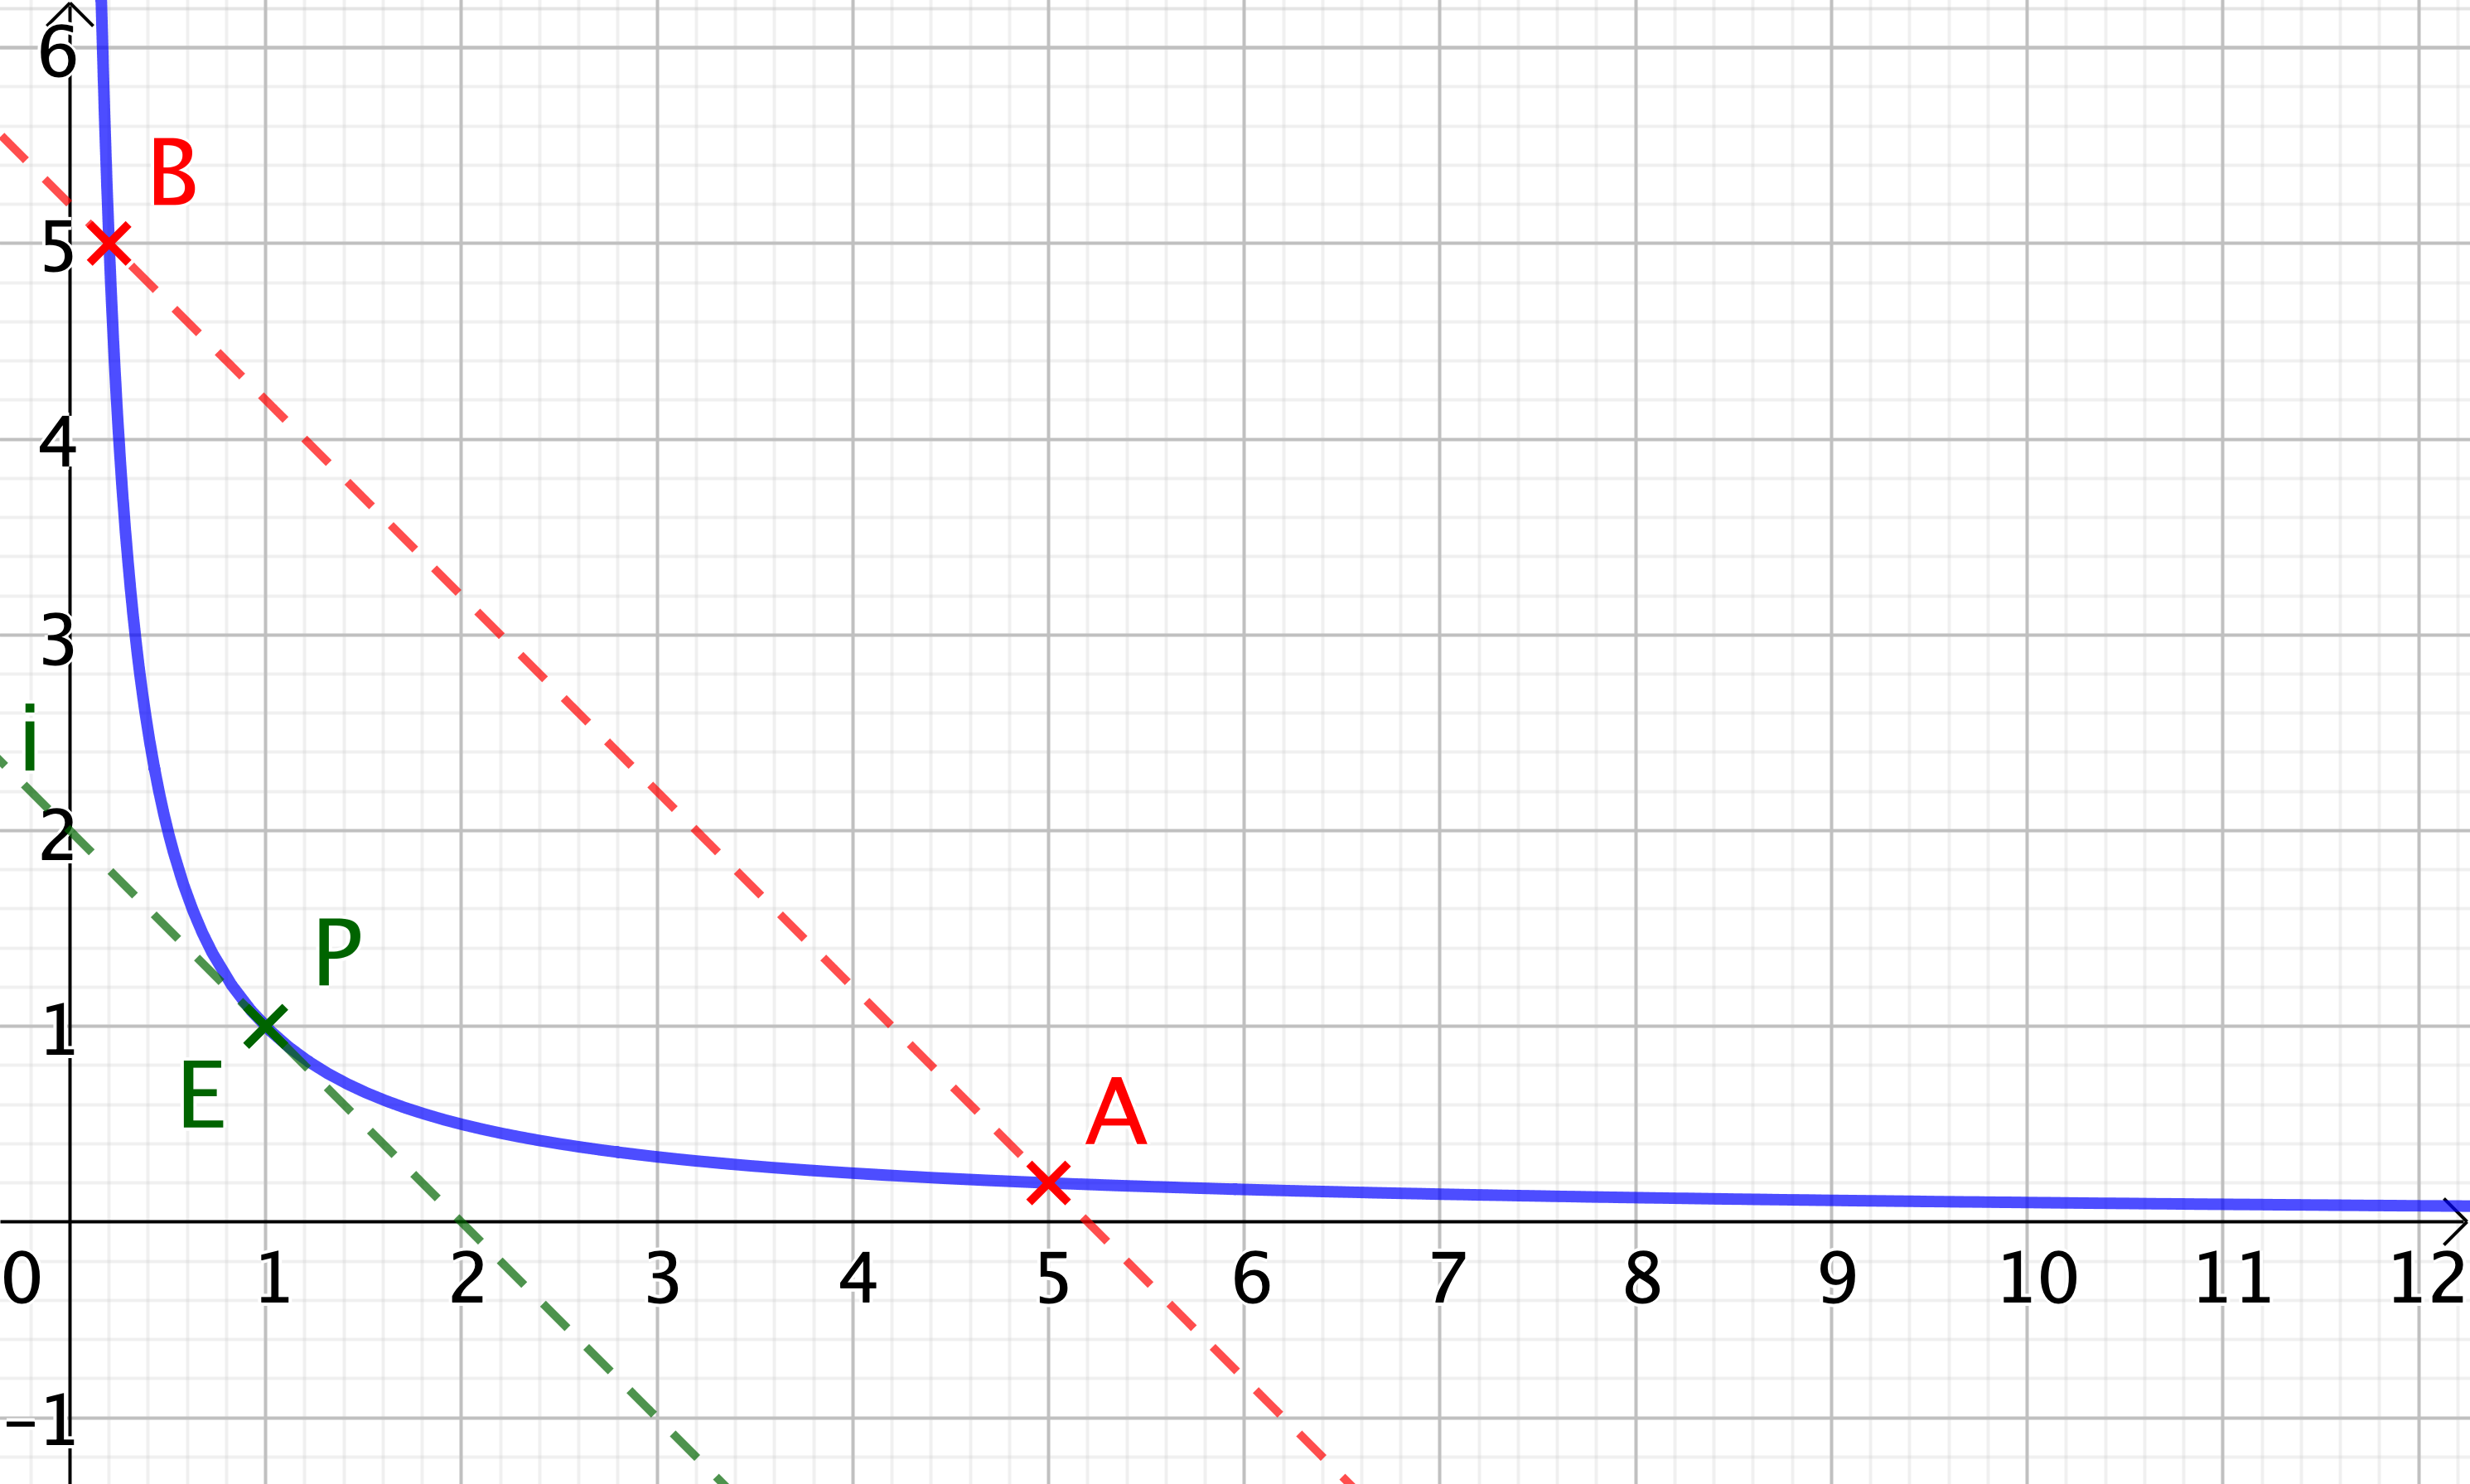
\includegraphics[scale = .75]{product-on-hyperbolas/conjecture/a-and-b-inverse-with-lines.png}}
	
	\smallskip
	Cas où $a b = 1$
\end{center}


\medskip

Il devient évident de conjecturer que le point $P$ se construit géométriquement comme suit.

\begin{enumerate}
	\item \label{point-1} Si $x_A x_B \neq 1$ et $A \neq B$ alors on construit la parallèle à $(AB)$ passant par $E$ . Le point $P$ est le second point d'intersection de cette parallèle avec $\setgeo{H}$  \emph{(notons qu'une droite coupe $\setgeo{H}$ en au plus deux points)}.

	\item Si $x_A x_B = 1$ alors $P = E$ . Notons au passage que l'on peut voir ceci comme un cas limite du précédent avec un point d'intersection \squote{double}.

	\item Si $x_A x_B \neq 1$ et $A = B$ , on procède comme au point (\ref{point-1}) mais avec la parallèle à la tangente en $A$ à l'hyperbole $\setgeo{H}$ .
\end{enumerate}


La section qui suit va valider cette conjecture qui donne un moyen très capillotracté de calculer un produit de deux réels non nuls via l'hyperbole $\setgeo{H}$ .
Plus sérieusement, la construction ci-dessus est une propriété géométrique très jolie de l'hyperbole $\setgeo{H}$ .
